\chapter{Calculation commands and scripting in Warteschlangensimulator}

\renewcommand{\thepage}{\arabic{page}}
\setcounter{page}{1}

\textbf{Calculation commands} can be used in the simulator e.g.\ to determine time periods
(such as processing times) or to specify in which branching direction a client should be directed.

\textbf{Scripts} can be used both for the determination of branch directions and for the evaluation
of simulation results and for running of parameter series. The Warteschlangensimulator uses
Javascript and Java as languages.



\section{Create expressions}

To the right of all input fields into which calculations commands can be entered
always the following button is displayed:
\fbox{
\includegraphics[width=0.25cm]{wand.png}}
By using this button the \textbf{Edit expression} dialog
(see figure \ref{fig:ExpressionBuilder}) can be accessed.
The dialog contains a complete list of all the commands available
in the current context, and makes it easy to put together
more complex commands and expressions.

\begin{figure}[ht]	
	\caption{Edit expression dialog}
	\centerline{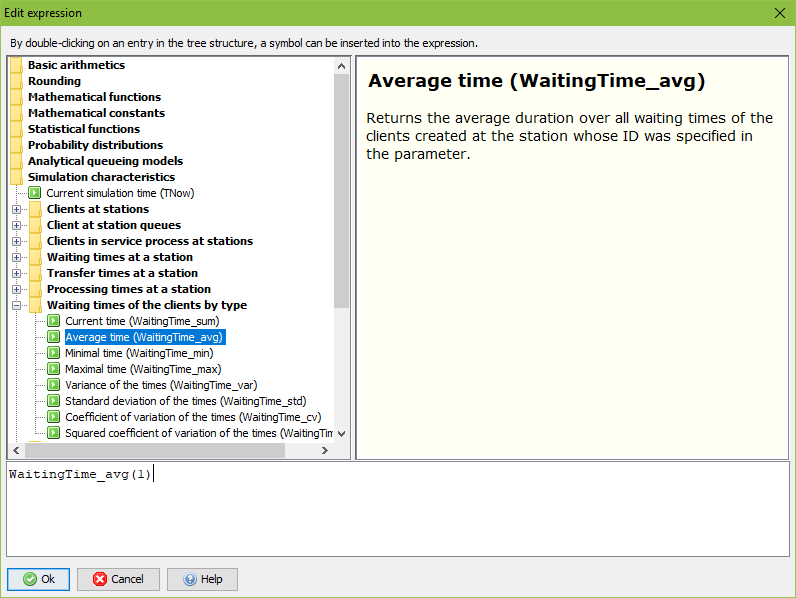
\includegraphics[width=14cm]{DialogExpressionBuilder.png}}
	\label{fig:ExpressionBuilder}
\end{figure}